\chapter{Rešerše používaných algoritmů}
\label{chap:reserzepouzivanychalgoritmu}
	Tato kapitola se zabývá přehledem využívaných algoritmů pro tvorbu polygonů z množiny linií. Polygonizace, tak jak jí můžeme pozorovat v různých GIS softwarech, se zpravidla neřeší jedním algoritmem, ale používají se různé algoritmy pro jednotlivé kroky polygonizace. Popíšeme zde tedy do jakých kroků lze polygonizaci rozdělit a jak jednotlivé kroky optimálně řešit. Budeme se zabývat i řešením v jednotlivých GIS softwarech.

	Polygonizaci lze nejjednodušeji rozdělit na 2 základní kroky. Jako vstupní data budeme uvažovat množinu linií, tyto linie ovšem nemusí obsahovat, v reálném použití převážně neobsahují, lomové body ve společných průsečících. V terminologii GIS se tyto průsečíky označují jako \textit{fuzzy}, volně přeloženo jako \textit{neostré}. Abychom mohli zahájit další krok polygonizace, je nutné tyto průsečíky doplnit. V první části se tedy budeme zabývat, jak optimálně doplnit průsečíky množin linií.
	
	Předpokládejme že množina linií je zbavená \textit{fuzzy} průsečíků, tedy každá dvojice úseček má společný nanejvýš jeden koncový bod. V takovéto situaci můžeme přistoupit k dalšímu kroku, tedy vlastní tvorbě polygonů z množiny linií. Polygony, které hledáme, musí splňovat podmínku, že žádný námi vytvořený polygon nemůže být rozdělen jakoukoliv linií na více menších polygonů. Pro řešení tvorby polygonů se často využívá grafových algoritmů.
	
\begin{figure}[h]
    \centering % <-- added
\begin{subfigure}{0.5\textwidth}
  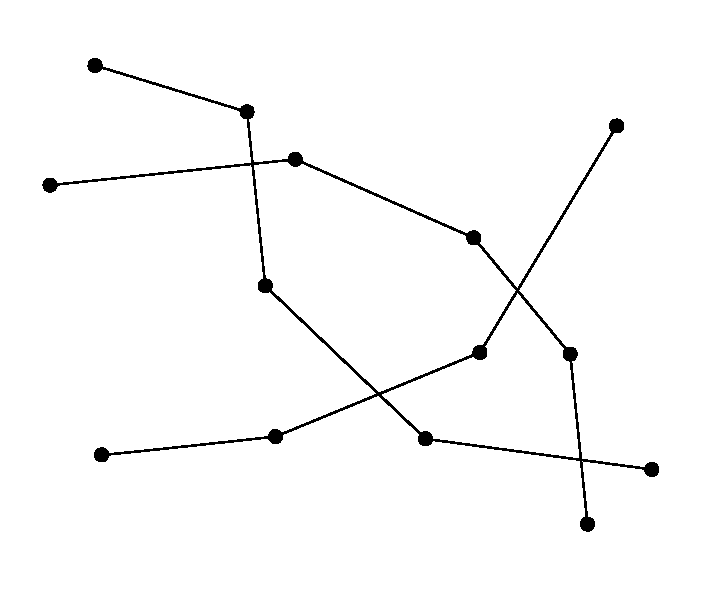
\includegraphics[width=\linewidth]{./pictures/2/fuzzy_1.pdf}
  \caption{Množina linií s fuzzy průsečíky}
  \label{fig:2-fuzzy_1}
\end{subfigure}\hfil % <-- added
\begin{subfigure}{0.5\textwidth}
  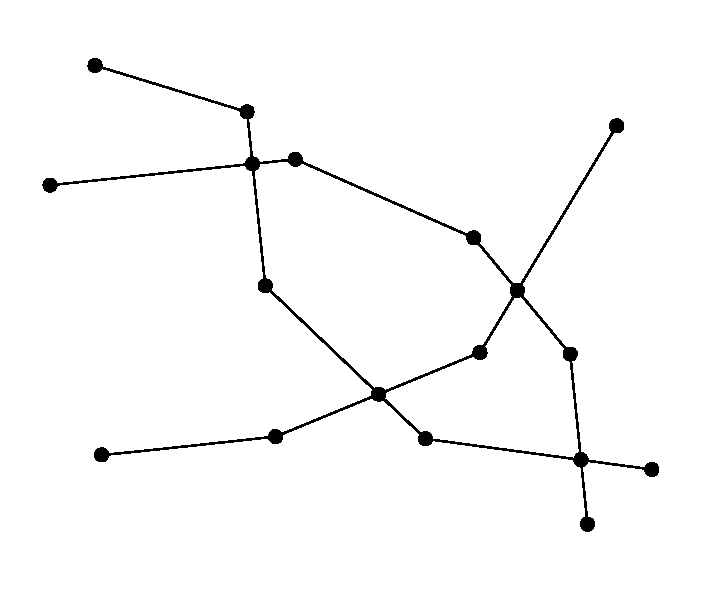
\includegraphics[width=\linewidth]{./pictures/2/fuzzy_2.pdf}
  \caption{Množina linií doplněná o průsečíky}
  \label{fig:2-fuzzy_2}
\end{subfigure}\hfil % <-- added
\begin{subfigure}{0.5\textwidth}
  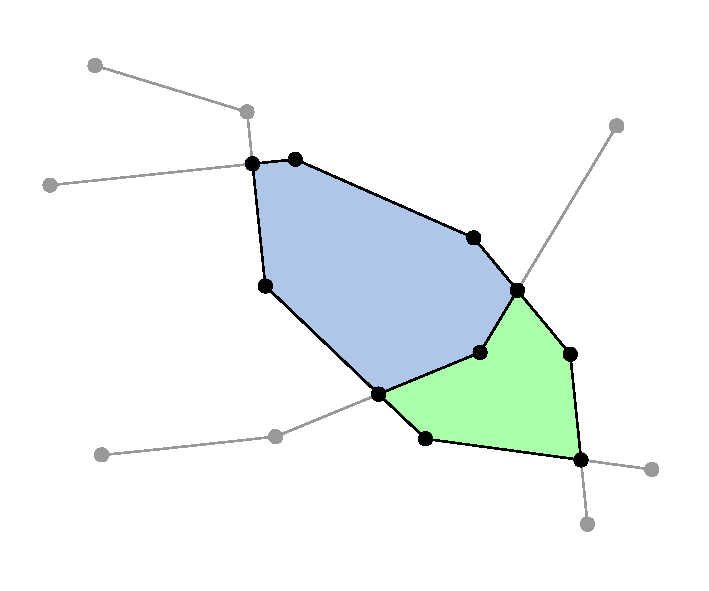
\includegraphics[width=\linewidth]{./pictures/2/fuzzy_3.pdf}
  \caption{Vytvořené polygony}
  \label{fig:2-fuzzy_2}
\end{subfigure}\hfil % <-- added
\caption{Znázornění postupu polygonizace}
\end{figure}

\section{Výpočet průsečíků množiny linií}
Výpočet všech průsečíků množin linií lze provést snadno, testováním všech úseček se všemi. Tímto postupem ovšem zjevně dosáhneme složitosti $\mathcal{O}(N^2)$. Pro výpočet průsečíků lze ovšem využít i algoritmus s časovou náročnosti $\mathcal{O}(n\log{}n)$, známý také jako Bentley–Ottmannův algoritmus \cite{bentley1979algorithms}.

\subsection{Vzájemná poloha dvou úseček}
Ve 2D výpočetní geometrii jsou standardně jednotlivé segmenty linie vyjádřeny počátečním a koncovým bodem. Uvažujme tedy že máme dány 2 přímky $p_1 = |S_1 E_1|$ a $p_2 = |S_2 E_2|$, kde $S_1 = [x_{S1},y_{S1}]$, $E_1 = [x_{E1},y_{E1}]$, $S_2 = [x_{S2},y_{S2}]$, $E_2 = [x_{E2},y_{E2}]$ a potřebujeme provést test, zda se dané přímky protínají či nikoliv, můžeme použít takzvaný \textit{Half-Plane} test, tedy test, který určuje zda bod leží v pravé či levé polorovině od přímky. Tento test zopakujeme celkem čtyřikrát a to na počáteční a koncový bod druhé úsečky, abysme zjistili zda se přímky protínají. Test je založen na výpočtu orientace dvou vektorů $\vec{u}$  a $\vec{v}$, kde vektor $\vec{v}$ je směrový vektor úsečky, tedy $\overrightarrow{S_1E_1}$ a vektor $\vec{v}$ je vektor $\overrightarrow{S_1S_2}$.	

\begin{figure}[h]
  \centering
  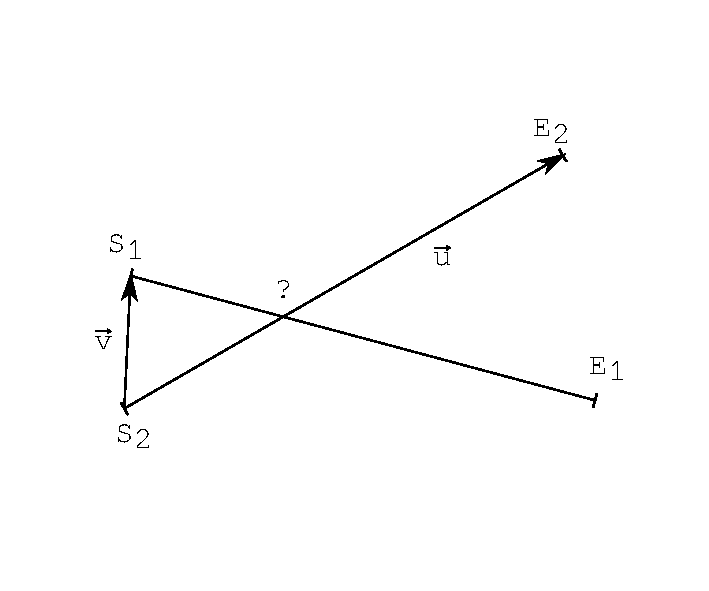
\includegraphics[width=7.5cm]{./pictures/2/half-plane_vector.pdf}
  \caption{\textit{Half-plane} test}
  \label{fig:2-half_plane_vector}
\end{figure}

\begin{figure}[h]
    \centering % <-- added
\begin{subfigure}{0.5\textwidth}
  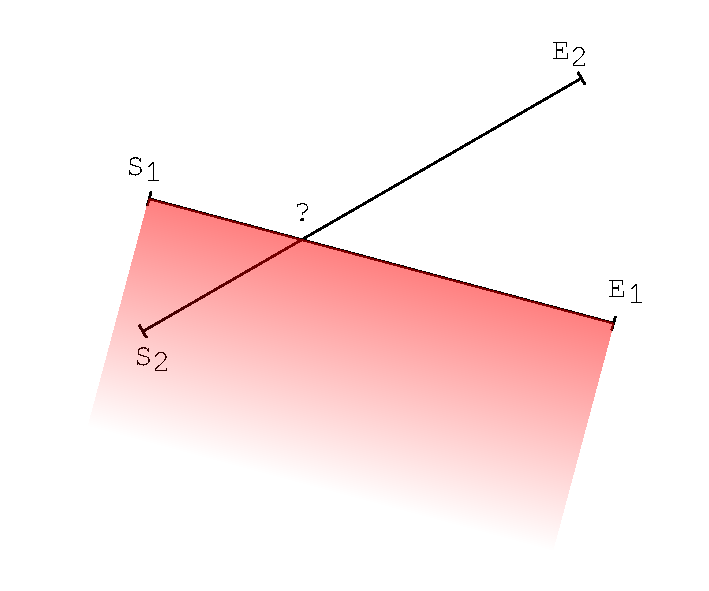
\includegraphics[width=\linewidth]{./pictures/2/half-plane_1.pdf}
  \caption{Test bodu $S_2$ k přímce $|S_1E_1|$}
  \label{fig:2-half_plane_1}
\end{subfigure}\hfil % <-- added
\begin{subfigure}{0.5\textwidth}
  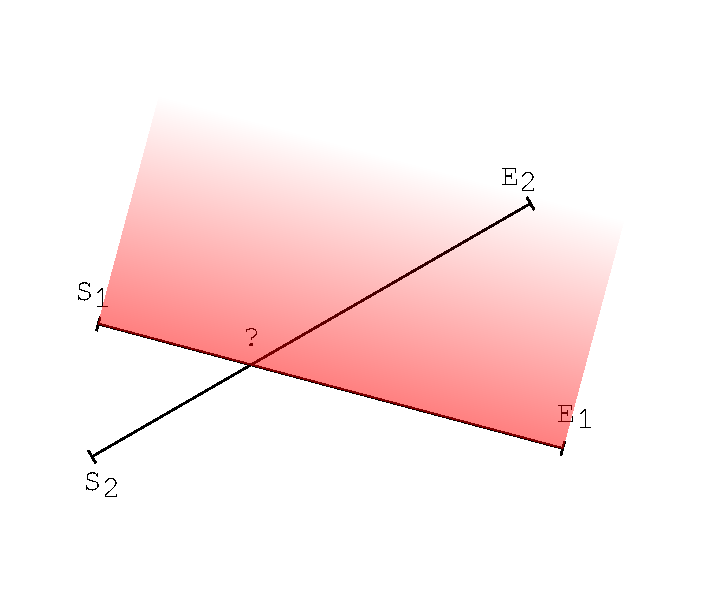
\includegraphics[width=\linewidth]{./pictures/2/half-plane_2.pdf}
  \caption{Test bodu $E_2$ k přímce $|S_1E_1|$}
  \label{fig:2-half_plane_2}
\end{subfigure}\hfil % <-- added

\medskip
\begin{subfigure}{0.5\textwidth}
  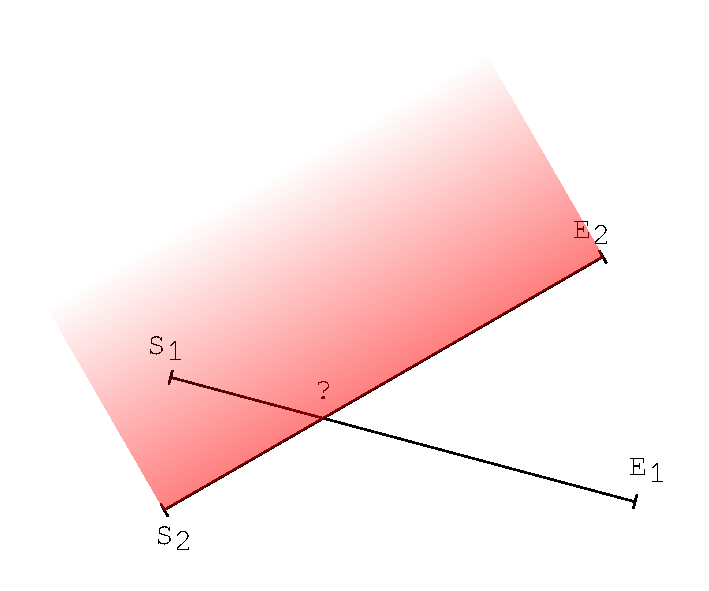
\includegraphics[width=\linewidth]{./pictures/2/half-plane_3.pdf}
  \caption{Test bodu $S_1$ k přímce $|S_2E_2|$}
  \label{fig:2-half_plane_3}
\end{subfigure}\hfil % <-- added
\begin{subfigure}{0.5\textwidth}
  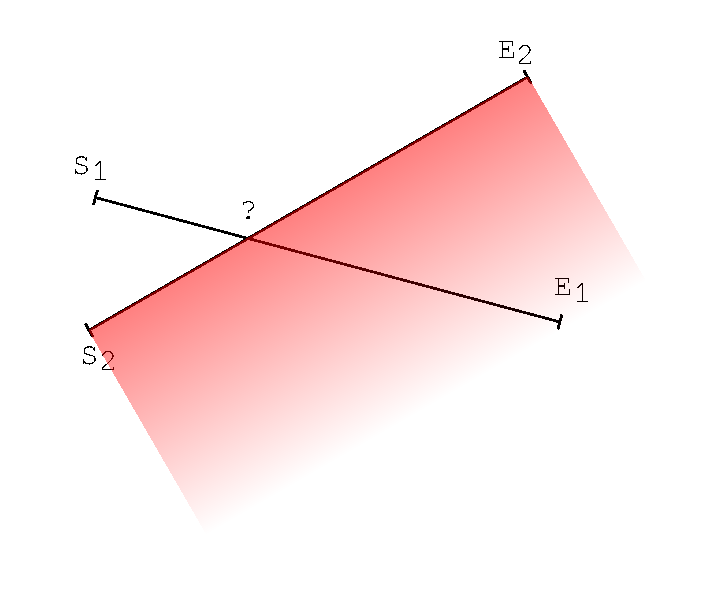
\includegraphics[width=\linewidth]{./pictures/2/half-plane_4.pdf}
  \caption{Test bodu $E_1$ k přímce $|S_2E_2|$}
  \label{fig:2-half_plane_4}
\end{subfigure}\hfil % <-- added
\caption{Grafické znázornění \textit{Half-plane} testů pro zjištění existence průsečíku}
\label{fig:2-half_plane}
\end{figure}

\subsection{Nalezení průsečíku dvou úseček}


\subsection{Bentley–Ottmannův algoritmus}
Tento algoritmus je založen na technice zvané \textit{sweep line}, překládané jako \textit{zametací přímka}, pro kterou je předpokladem mít setříděná vstupní data, podle jedné ze souřadnic. Algoritmus zde nebuda více popisován jelikož je velmi dobře vysvětlen v těchto publikacích \cite{bentley1979algorithms} \cite{bayer2008algoritmy}.

\section{Tvorba polygonů z množiny linií}
Předpokládejme že máme množinu linií doplněnou o průsečíky, tedy každá dvojice úseček v této množině sdílí nejvýše jeden koncový bod. V předchozí sekci bylo řečeno že průsečíky linií lze doplnit pomocí \textit{Bentley–Ottmannova} algoritmu v čase $\mathcal{O}(n\log{}n)$. Nyní chceme tedy v této množině linií nalézt všechny polygony, tak aby jednotlivé polygony spolu sdílely maximálně hrany a zároveň aby žádný z polygonů nemohl obsahovat jiný polygon.
	
\subsection{Nalezení všech cyklů v grafu}




Jak již bylo řečeno, polygonizace se provádí nad daty s doplněnými průsečíky linií. Doplnění průsečíku jsme schopni vyřešit v čase $\mathcal{O}(n\log{}n)$. Nyní tedy nastává otázka jak řešit vlastní polygonizaci.


\section{GIS software}
Provedení polygonizace zvládá většina současně používaného GIS softwaru. Pokusíme se tedy rozebrat postupy jednotlivých nástrojů na polygonizaci.

\subsection{ArcGIS}
ArcGIS je vyvíjený společností Esri, v současné době se jedná o nejpokročilejší nástroj v oblasti GIS. Jedná se o proprietární software, u kterého 


\subsection{QGis}
QGis je nejspíše jeden z nejznámějších volných nástrojů pro práci v GIS. Je šířen pod copyleftovou  licencí \textit{GNU General Public License}, tudíž máme volný přístup ke zdrojovému kódu aplikace dostupných v online repozitářích. To nám umožňuje nahlížet do výpočetních algoritmů, které jsou v případě QGis psány v programovacím jazyce \textit{C++} a \textit{Python}, narozdíl od komerčních nástrojů, které si implementaci často chrání

\subsection{Grass GIS}

\subsection{PostGis}
